% environment.tex

\section{Simulation Environment}
\label{sec:env}

This section describes the dynamic decentralized FANET simulation environment. The environment models a swarm of $N$ UAVs with decentralized cluster formation, cross-layer multi-fading channel effects (supporting AWGN, Rayleigh, Rician, and Nakagami distributions), and time-burst split MAC control.

\begin{figure*}[t]
    \centering
    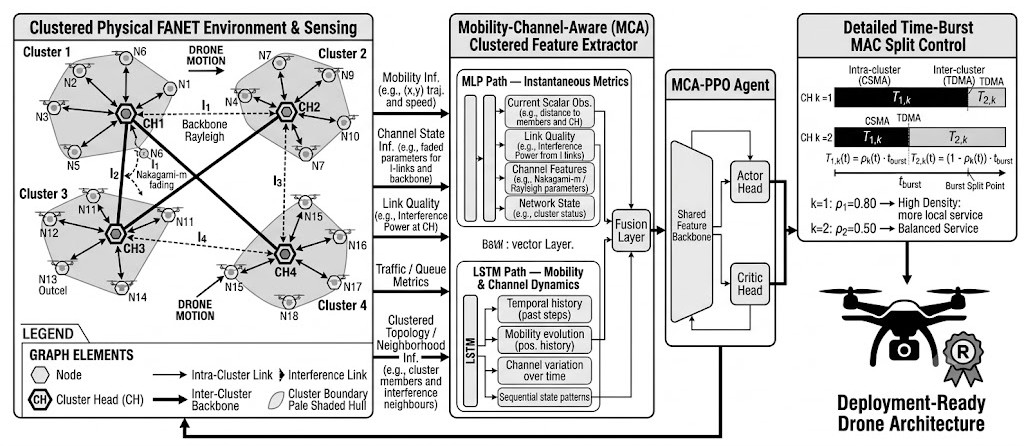
\includegraphics[width=\textwidth, height=6.5cm]{figures/pipeline_2.jpg}
    \caption{Combined FANET Clustering and MCA-based Time-Burst MAC Control Diagram. This comprehensive architecture illustrates: (1) The decentralized dynamic FANET clustering graph; (2) The time-burst MAC split control structure bridging intra-cluster CSMA access and inter-cluster TDMA coordination; (3) The heterogeneous multi-fading channels experienced by the drone swarm; (4) The MCA Feature Extractor processing mobility and channel dynamics via fused MLP and LSTM paths; and (5) The final MCA-PPO Agent directing deployment-ready drone transmission policies.}
    \label{fig:comprehensive_pipeline}
\end{figure*}

\subsection{Decentralized Clustered Topology}

Consider a FANET of $N = 50$ UAVs operating within a three-dimensional bounding volume. At each decision instant~$t$, the swarm is partitioned into $c(t)$ non-overlapping clusters:
\begin{equation}
    \mathcal{U}(t) = \bigcup_{k=1}^{c(t)} \mathcal{C}_k(t), \quad \mathcal{C}_k(t) \cap \mathcal{C}_\ell(t) = \emptyset,\; k \neq \ell.
    \label{eq:partition}
\end{equation}
Each cluster $\mathcal{C}_k(t)$ is managed by a cluster-head $L_k(t) \in \mathcal{C}_k(t)$. The suitability of node $i$ to serve as a cluster-head, referred to as the \textit{Cluster-Head Health} score, is evaluated using a weighted composite score:
\begin{align}
    H_i(t) =\; & w^h_{\text{energy}} \bar{E}_i(t) + w^h_{\text{degree}} \bar{D}_i(t) + w^h_{\text{mob}} M_i(t) \nonumber \\
    & - w^h_{\text{queue}} \bar{Q}_i(t) - w^h_{\text{risk}} R_i(t),
    \label{eq:ch_score}
\end{align}
where $\bar{E}_i(t)$ is normalized residual energy, $\bar{D}_i(t)$ is normalized node degree, $M_i(t)$ is mobility stability, $\bar{Q}_i(t)$ is queue occupancy, and $R_i(t)$ is link breakage risk. This Health score explicitly tracks the structural stability of the cluster across time.

Subordinate nodes select their cluster-head based on a membership score $S_{i,k}(t)$ derived from distance and link quality. A UAV reassociates from cluster $u$ to cluster $v$ only when the score difference exceeds a hysteresis threshold:
\begin{equation}
    S_{i,v}(t) - S_{i,u}(t) \geq \Delta_{\text{reasoc}},
    \label{eq:hysteresis}
\end{equation}
which prevents oscillatory ping-pong effects during border traversal.

\subsection{System Model and Multi-Fading Channel}

Packet arrivals for each UAV follow an independent Poisson process with a configurable mean rate $\lambda$ (packets/sec). The fundamental service model operates over communication bursts of duration $t_{\text{burst}}$. Air-to-air links are heavily influenced by 3D mobility and multi-path fading. Large-scale path loss is captured via the free-space path loss model, $PL(d) = 20\log_{10}(d) + 20\log_{10}(f) + 20\log_{10}(4\pi/c)$ in dB. For small-scale fading, the environment supports AWGN, Rayleigh, Rician, and Nakagami distributions depending on line-of-sight conditions. For mathematical concreteness, under the Nakagami-$m$ distribution, the probability density function (PDF) of the received power $p$ is:
\begin{equation}
    f_P(p) = \left( \frac{m}{\Omega} \right)^m \frac{p^{m-1}}{\Gamma(m)} \exp\left( - \frac{m p}{\Omega} \right), \quad p \geq 0,
    \label{eq:nakagami}
\end{equation}
where $\Gamma(\cdot)$ is the Gamma function, $\Omega = \mathbb{E}[P]$ is the average received power, and $m$ is the fading figure. Assuming QPSK modulation over a 5\,Mbps physical layer, the theoretical bit-error rate is evaluated as $P_b \approx Q(\sqrt{\text{SINR}})$. Packets are strictly counted as \textit{drops} if they fall into one of three categories: (1) experiencing a BER exceeding $10^{-3}$, (2) suffering unrecoverable MAC-layer collisions during CSMA/CA contention (due to overlapping transmissions or hidden terminal effects), or (3) encountering queue overflow in the finite drone transmission buffers.

\begin{figure}[t]
    \centering
    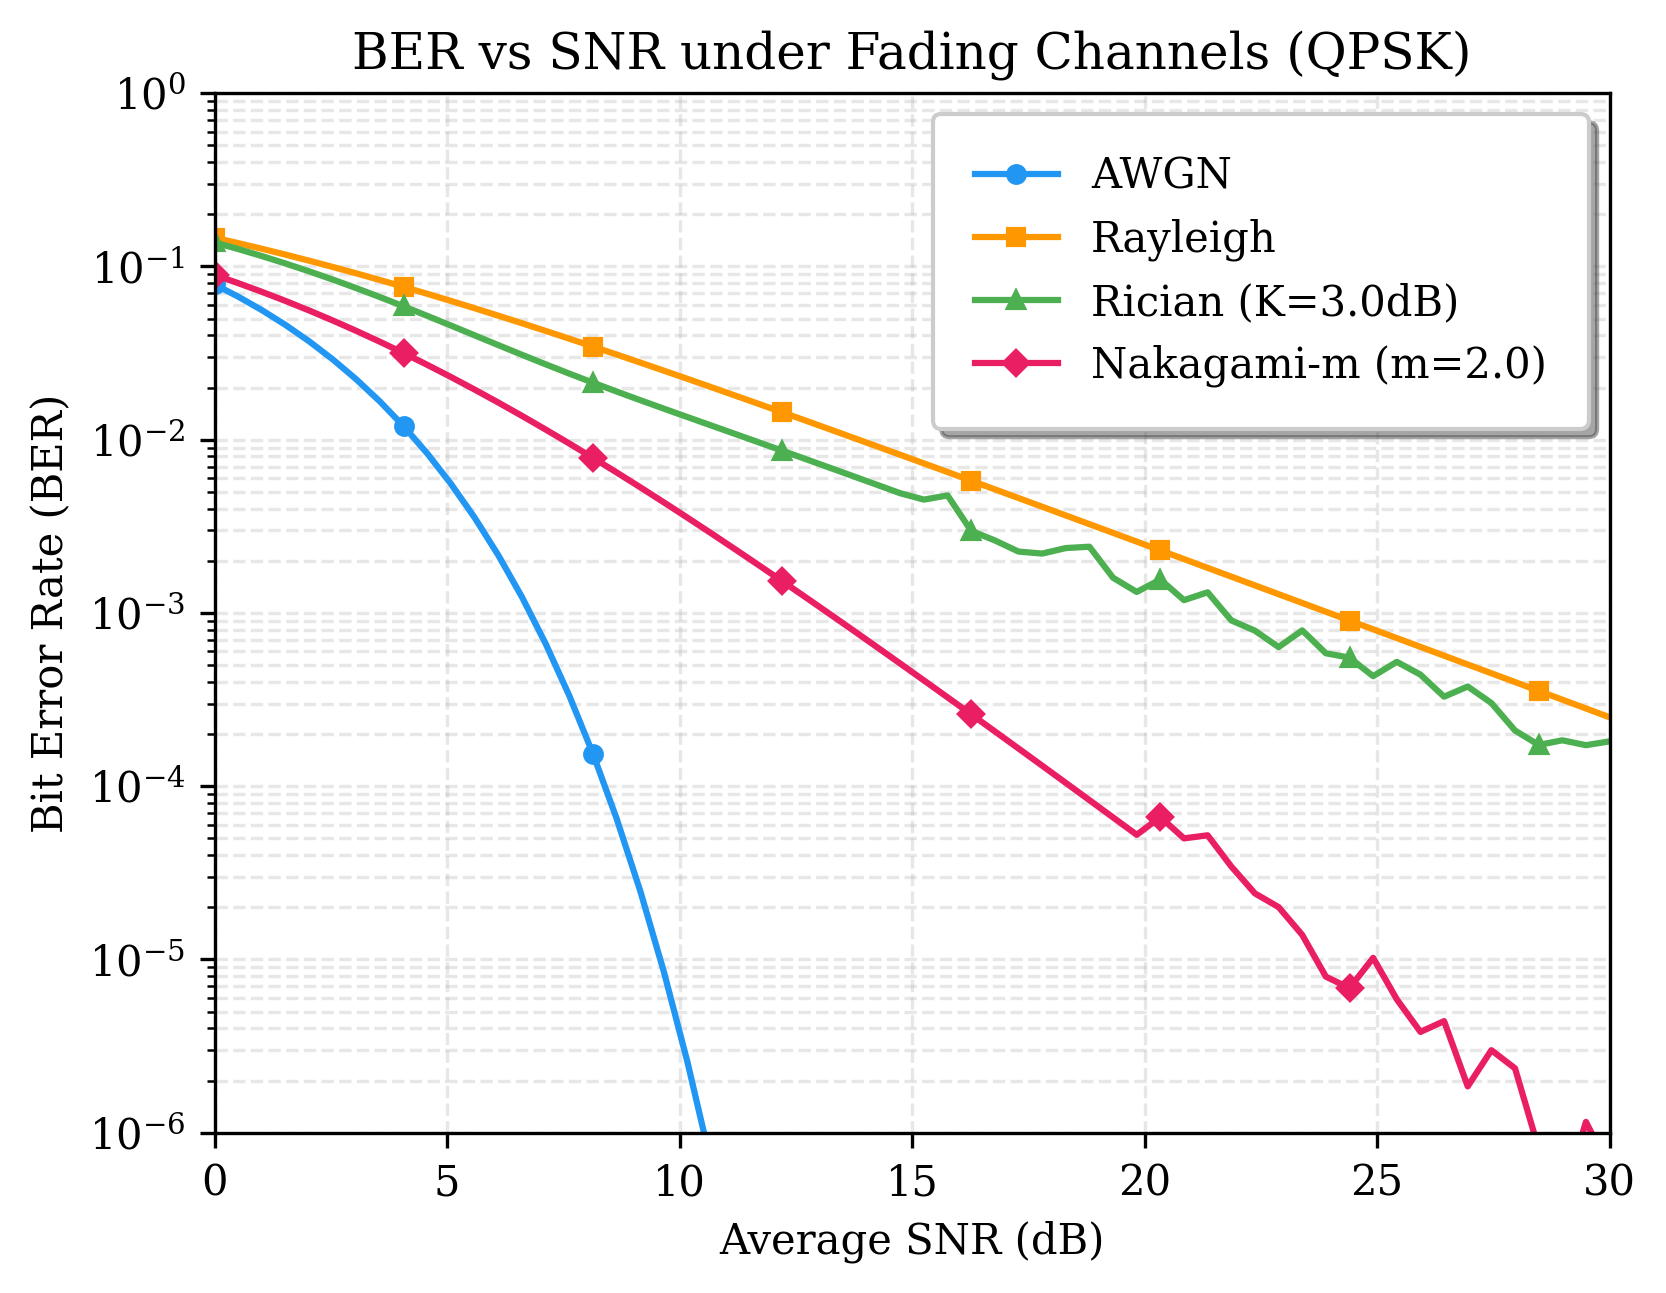
\includegraphics[width=\columnwidth]{figures/ber_snr_fading.png}
    \caption{BER--SNR behavior under QPSK fading channels. The environment supports AWGN, Rayleigh, Rician, and Nakagami-$m$ fading conditions.}
    \label{fig:ber_snr}
\end{figure}

\subsection{Time-Burst Split MAC Control}

To adapt to the dynamically shifting intra-cluster vs. inter-cluster traffic demands, the environment implements a time-burst split MAC protocol as illustrated in Figure~\ref{fig:comprehensive_pipeline}. At each control interval, the RL agent governing the cluster selects a joint action:
\begin{equation}
    a(t) = \big(m(t),\; \rho(t)\big).
    \label{eq:action}
\end{equation}
The discrete mode $m(t) \in \{0, 1\}$ shifts the fundamental access strategy: $m(t)=0$ triggers a scheduled TDMA access frame, whereas $m(t)=1$ triggers a contention-based CSMA/CA period. 
Simultaneously, the continuous time-burst ratio $\rho(t) \in [0,1]$ splits the total communication burst duration $t_{\text{burst}}$ into two segments:
\begin{align}
    T_{\text{intra}}(t) &= \rho(t) \cdot t_{\text{burst}}, \label{eq:T1} \\
    T_{\text{inter}}(t) &= (1 - \rho(t)) \cdot t_{\text{burst}}, \label{eq:T2}
\end{align}
where $T_{\text{intra}}(t)$ is strictly allocated for cluster-head to subordinate communication, and $T_{\text{inter}}(t)$ is reserved for inter-cluster routing.



\subsection{Reward Function and Jain's Fairness}

The RL reward signal aggregates four performance metrics, normalized to $[0,1]$ against theoretical bounds:
\begin{equation}
    R_t = w_T \bar{T}(t) - w_D \bar{D}(t) - w_F \bar{F}(t) - w_J \bar{C}(t),
    \label{eq:reward}
\end{equation}
where $\bar{T}(t) = T(t) / R_{\text{PHY}}$ is the normalized throughput, $\bar{D}(t) = D(t) / D_{\max}$ is the normalized end-to-end delay, $\bar{F}(t)$ is the packet drop ratio, and $\bar{C}(t)$ is the normalized collision count. These weights ($w_T, w_D, w_F, w_J$) are tuned via Optuna.

To evaluate load-balancing equity across the decentralized clusters, we utilize Jain's Fairness Index:
\begin{equation}
    J(x) = \frac{\left( \sum_{i=1}^{N} x_i \right)^2}{N \sum_{i=1}^{N} x_i^2},
    \label{eq:jains}
\end{equation}
where $x_i$ represents the measured throughput of UAV $i$. A value of $J \approx 1$ indicates perfectly fair resource allocation across the network.


\begin{table}[t]
    \centering
    \caption{Simulation environment parameters. The environment models a 50-node dynamic FANET with multi-fading channel conditions.}
    \label{tab:sim_params}
    \begin{tabular}{@{}lc@{}}
        \toprule
        \textbf{Parameter} & \textbf{Value} \\
        \midrule
        Number of UAVs ($N$) & 50 \\
        PHY data rate ($R_{\text{PHY}}$) & 5\,Mbps \\
        Modulation & QPSK \\
        Fading model & Multi-Fading \\
        BER threshold & $10^{-3}$ \\
        Mobility model & Circular/spiral \\
        Speed range $[V_{\min}, V_{\max}]$ & $[5, 35]$\,m/s \\
        Bounding volume & $200 \times 200 \times 50$\,m \\
        Queue capacity ($Q_{\max}$) & 100 packets \\
        Packet payload & 1000\,bytes \\
        Traffic sweep & 50--1000\,pps \\
        Decision interval & 1.0\,s \\
        \bottomrule
    \end{tabular}
\end{table}
